%FEBRUARY 2020, made by the TeXniCie with input from Freek Geerligs
\documentclass{beamer}

\usetheme{aes2}
%\usetheme{Frankfurt} %A different but comparable theme if you don't want to use the aeskwadraat theme

% Packages:
%\usepackage[a4paper]{geometry} 
\usepackage[english]{babel} %for correct linebreaks
\usepackage{parskip} % Alineas start on the left and there is an empty line between alineas.
\usepackage{amsmath, amssymb, textcomp,amsthm} % Mathematical symbols etc
\usepackage{color}
\usepackage{enumerate}
\usepackage{hyperref} %For hyperlinks that you can click on

\usepackage {graphicx} % To include pictures
\usepackage{caption}
%\usepackage{subcaption}
%\usepackage{subfig}

\usepackage{mathrsfs}
\usepackage{amsthm}% For definition, proof, theorem etc environments.

\usepackage{tikz-cd}

%Here some lines for layout of theorems and enumerate them well
\theoremstyle{definition}
\newtheorem{dfn}{Definition}[section]% enumeration now follows sections
\theoremstyle{example}
\newtheorem{conseq}[dfn]{Consequence}
\newtheorem{const}[dfn]{Construction}
%\theoremstyle{plain}
\newtheorem{thm}[dfn]{Theorem}% enumeration now follows definitions 
%\newtheorem{lemma}[dfn]{Lemma}
%\newtheorem{example}[]{Example}
%\newtheorem{nexample}[example]{Non-example}


%\usecolortheme{dolphin} %crane of dolphin
%\useinnertheme{circles}
%\useoutertheme{smoothbars}

\title{Title of your presentation}
\date{\today}
\author{Your name here}

\begin{document}

\begin{frame}
\titlepage
\end{frame}	

\begin{frame}{Contents} %What is on a slide is in the frame environment, you can name each slide
	\tableofcontents
\end{frame}
\section{First subject}
%The structure (sections, subsections etc) you're used to in TeX-files can still be used, you can see the structure in the table of contents and in the progress-bar at the top of each slide.


\begin{frame}
	\frametitle{What everyone should know before I start}
	In the frame environment you can do what you are used to in \LaTeX. For example nice formulas like
	\begin{align}
	E &= \frac{p^2}{2m}\\
	E_{rel}^2 &= m^2c^4 + p^2c^2
	\end{align}
	\begin{block}{Important}
		It is \quad I M P O R T A N T \quad to be able to \textbf{emphasise} \textit{in different} \emph{ways}!
	\end{block}
 
\end{frame}

\begin{frame}{Let's continue}
Sometimes it is a shame if everything you want to say is already on the slide.\newline
\begin{thm}
	You do not yet know the proof of this theorem.
\end{thm}
\begin{block}{Proof}
	The proof is here.
\end{block}
But we can fix this!\\
Let's try this again.

\end{frame}

\subsection{This subsection is not in the progress bar but is in the table of contents!}

\begin{frame}{Again!}
\begin{thm}
	You do not yet know the proof of this theorem.
\end{thm}
\pause
\begin{block}{Proof}
	The proof is here.
\end{block}
\pause
Much better!
\end{frame}

\section{Applications}

\begin{frame}{More advanced}
	\only<1->{We can even make the text disappear.\\}
	\only<2-3>{Peekaboo!\\}
	\only<3>{Go and seek! (by lack of a better translation of \textit{Wie niet weg is is gezien!})}
	\only<4>{And let's go on...}
\end{frame}

\begin{frame}
Enumerations can look better this way as well
\begin{itemize}
	\only<1-2>{\item 1...}
	\only<2-3>{\item 2...}
	\only<3-4>{\item 3...}
	\only<4-5>{\item 4, 5, 6, 7, 8}
	\only<5-6>{\item 9...}
	\only<6>{\item 10!}
	\only<7>{\item Ready or not here I come!}
\end{itemize}

\end{frame}

%\begin{frame}{Even more advanced, taken from a thesis presentation}
%
%\begin{columns}[T] % align columns
%	\uncover<6->{	\begin{column}{.48\textwidth}
%			\begin{dfn}
%				For $x,y\in \hat R$, we define 
%				the \textbf{Kuratowski-tuple } $(x,y)$ as
%				$$(x,y):=\big\{\{x\},\{x,y\}\big\}$$ 
%			\end{dfn}
%	\end{column}}%
%	
%	\begin{column}{.48\textwidth}
%		
%	\begin{block}{The superstructure}
%	\begin{itemize}
%		\item			$R_0:=\mathbb R$. 
%		\item			$R_{n+1}:=\mathcal P(\bigcup\limits_{k=0}^nR_{k}),$ 
%		\item			$\hat R:= \bigcup\limits_{n\in\mathbb N} R_n$.
%	\end{itemize}
%\end{block}
%	\end{column}%
%	\hfill%
%
%
%\end{columns}
%\pause
%\begin{align*}
%	\uncover<3->{0,1,2 & \in }R_0	=\mathbb R
%	\\
%\uncover<4->{	\mathbb N, \mathbb Z, \mathbb Q, \mathbb R,\{0\},\{0,1\}&\in }R_1	=\mathcal P(\mathbb R)
%	\\ 
%\uncover<5->	{\mathcal T_{eucl}, \big\{\{0\},\{0,1\}\big\}&\in} R_2 =\mathcal P(\mathbb R\cup \mathcal P(\mathbb R))
%	\\
%\uncover<7->	{   \mathbb R^2, \{(x,x+1)|x\in\mathbb R \}, \{(x,y)|x\leq y\}&\in }R_3 =\mathcal P(R_0\cup R_1\cup R_2)
%\\
%\uncover<8->	{  C^\infty(\mathbb R), \mathbb R^\mathbb R, \mathbb R^\mathbb N&\in }R_4 =\mathcal P(R_0\cup R_1\cup R_2\cup R_3)\end{align*}
%
%
%\end{frame}



\begin{frame}
\begin{columns}[T]
	\begin{column}[T]{5cm}
		We can also place colums next to each other.\\
		\begin{block}{Also cool}
			More indents in your code.
		\end{block}
		\begin{alertblock}{Attention!}
			A block for even more \emph{emphasis}!\\
			Just differently colored.
		\end{alertblock}
	\end{column}
	\begin{column}[T]{5cm}
		We can even include pictures!
		\begin{figure}
			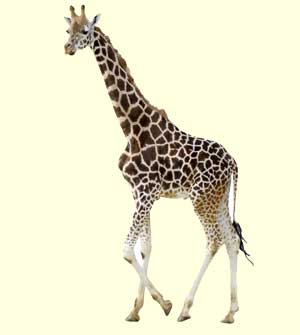
\includegraphics[scale=0.4]{Giraffe_klein.jpg}
			\caption{A picture you might recognise.}
		\end{figure}
		
	\end{column}
\end{columns}
\end{frame}


\section{Also}


\begin{frame}{Also}
Don't forget to compile, the table of contents and the progress bar will need more than one compilation to be updated correctly.\\
At the end of a presentation you thank your audience and leave room for questions.\\
Then your presentation is done!
\end{frame}

\end{document}